\documentclass[aspectratio=169,11pt]{beamer}
\usepackage[utf8]{inputenc}
\usepackage[T1]{fontenc}
\usepackage{lmodern,graphicx,amsmath,booktabs}
\usepackage{xcolor,tikz}
\usepackage{pgfpages}
\usetikzlibrary{arrows.meta,positioning,calc,fit,shapes.geometric}

% Presenter mode: the compiled PDF shows each slide on the left and its
% transcript on the right. Change \presenternotestrue to
% \presenternotesfalse to compile the normal audience slides only.
\newif\ifpresenternotes
\presenternotestrue
%\presenternotesfalse
\ifpresenternotes
  \setbeameroption{show notes on second screen=right}
\else
  \setbeameroption{hide notes}
\fi

% Visual language retained from the supplied research-ideas template.
\definecolor{tumblue}{RGB}{0,101,189}
\definecolor{tumdark}{RGB}{0,51,89}
\definecolor{tumgray}{RGB}{105,105,105}
\definecolor{tumlight}{RGB}{235,243,248}
\definecolor{tumgreen}{RGB}{162,173,0}
\definecolor{tumorange}{RGB}{243,125,32}
\definecolor{tumred}{RGB}{229,52,24}
\definecolor{zeogray}{RGB}{218,213,202}
\definecolor{poreblue}{RGB}{94,181,226}
\definecolor{co2blue}{HTML}{2C7FB8}

\usetheme{default}
\setbeamertemplate{navigation symbols}{}
\setbeamercolor{normal text}{fg=black,bg=white}
\setbeamercolor{frametitle}{fg=tumblue}
\setbeamercolor{structure}{fg=tumblue}
\setbeamercolor{itemize item}{fg=tumblue}
\setbeamertemplate{itemize items}[circle]
\setbeamertemplate{headline}{%
  \leavevmode\begin{beamercolorbox}[wd=\paperwidth,ht=3.2ex,dp=1.6ex]{frametitle}
  \hfill\raisebox{-0.85cm}{
\includegraphics[height=0.8cm]{figures/tum_logo.png}}\hspace*{1em}
  \end{beamercolorbox}}
\setbeamertemplate{footline}{%
  \leavevmode\begin{beamercolorbox}[wd=\paperwidth,ht=3.2ex,dp=1.3ex]{author in head/foot}
  \hspace*{1em}\color{tumgray} Khalifa and Briesen \enspace|\enspace PoreAccess--CO$_2$
  \hfill\insertsectionhead\hfill\insertframenumber/\inserttotalframenumber\hspace*{1em}
  \end{beamercolorbox}}

\newcommand{\hi}[1]{\textcolor{tumblue}{\textbf{#1}}}
\newcommand{\question}[1]{%
  \begin{beamercolorbox}[rounded=true,sep=0.65em]{block body}
  \centering\large\color{tumdark}\textbf{#1}
  \end{beamercolorbox}}
\newcommand{\result}[1]{%
  \begin{beamercolorbox}[rounded=true,sep=0.55em]{block body}
  \centering\color{tumdark}\textbf{#1}
  \end{beamercolorbox}}
\newcommand{\source}[1]{\par\vfill{\tiny\color{tumgray}Source: #1}}
\tikzset{
  box/.style={draw=tumdark!75,rounded corners=2pt,fill=tumlight,
    align=center,minimum height=9mm,text width=2.55cm,font=\small,inner sep=3pt},
  arr/.style={-{Latex[length=2mm]},thick,tumblue},
  bead/.style={circle,draw=black!65,fill=zeogray,minimum size=6.4mm,inner sep=0pt},
  pore/.style={circle,draw=tumblue!80!black,fill=poreblue,minimum size=1.8mm,inner sep=0pt},
  throat/.style={draw=tumblue!82,line width=1.05pt}}

\newcommand{\FlexRowHeight}{}
\newenvironment{FlexRow}[1]{%
  \def\FlexRowHeight{#1}\begin{overlayarea}{\textwidth}{#1}\begin{columns}[T,onlytextwidth]
}{\end{columns}\end{overlayarea}}
\newcommand{\Col}[2]{\column{#1\textwidth}\begin{minipage}[t][\FlexRowHeight]{\linewidth}#2\end{minipage}}

\begin{document}

% -----------------------------------------------------------------------------
\begin{frame}{}
  \vspace*{0.2cm}
  \begin{FlexRow}{0.16\textheight}
    \Col{1.0}{\centering{\Large\bfseries PoreAccess--CO$_2$:}\\[0.7ex]
      {\Large\bfseries From Random Packing to an Interpretable Transport Closure}}
  \end{FlexRow}
  \vspace{0.45cm}
  \begin{FlexRow}{0.67\textheight}
    \Col{0.57}{\vspace{0.7cm}
      {\color{tumblue}\textbf{Structure-resolved diffusion and adsorption in DEM-generated zeolite beds}}\par
      \vspace{0.55cm}
      Technical University of Munich\\
      Chair of Process Systems Engineering\\[0.55cm]
      Ali Khalifa \& Heiko Briesen}
    \Col{0.40}{\vspace{0.08cm}\centering
      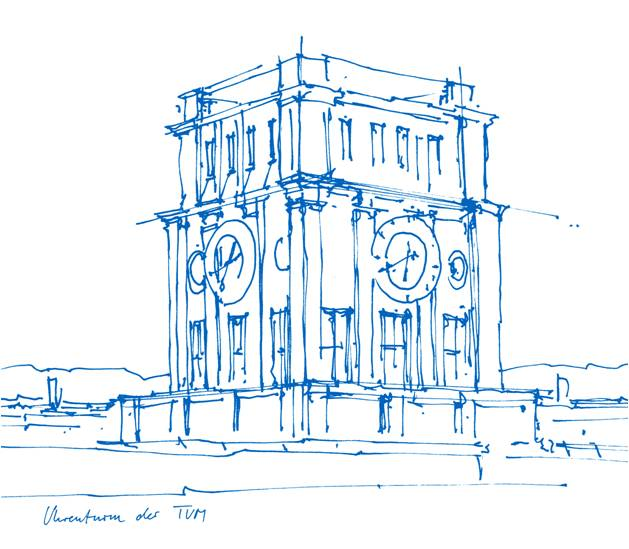
\includegraphics[width=1.03\linewidth,height=4.55cm,keepaspectratio]{figures/uhrenturm.jpg}}
  \end{FlexRow}
  \note{
    Good morning. This project is called PoreAccess--CO$_2$. It examines how
    the random arrangement of particles changes CO$_2$ transport through a
    packed zeolite bed. The main aim is to retain information about the pore
    structure while developing a model that is much faster than a complete
    pore-network adsorption simulation. I will first introduce the physical
    problem, then explain the pore-network and one-dimensional models. Finally,
    I will show how we connect them through an accessibility-based transport
    closure and what the first twenty packing realizations tell us.
  }
\end{frame}

\begin{frame}{Presentation outline}
\tableofcontents
\note{The presentation moves from the research question to the physical model, numerical methods, results and conclusions.}
\end{frame}

\section[Motivation]{Motivation and research question}
\begin{frame}{}
\vfill
{\large\color{tumgray}Section 1 of 5}\par\vspace{0.4cm}
{\LARGE\color{tumblue}\textbf{Motivation and research question}}\par\vspace{0.5cm}
{\large Why can similar beds adsorb differently?}
\vfill
\note{Why can similar beds adsorb differently?.}
\end{frame}

\begin{frame}{CO$_2$ adsorption matters and packing structure is a missing scale}
  \small
  \begin{columns}[T,onlytextwidth]
    \column{0.47\textwidth}
      \hi{Why CO$_2$ capturing matters?}
      \begin{itemize}
        \item Food systems contribute about \textbf{one-third} of global
              anthropogenic greenhouse-gas emissions.
        \item Food and bioprocessing include recoverable biogenic CO$_2$
              streams, for example from fermentation.
        \item Regenerable sorbents offer a compact capture and purification route.
      \end{itemize}
    \column{0.49\textwidth}
      \hi{What is already established?}
      \begin{itemize}
        \item CO$_2$ equilibrium and uptake kinetics on zeolite 13X are widely studied.
        \item Fixed-bed models normally use bulk porosity and a fitted
              effective transport coefficient.
        \item Random inlet-connected paths remain hidden inside that coefficient.
      \end{itemize}
  \end{columns}
  \vspace{0.18cm}
  \result{Novelty: connect random particle geometry to a fast bed-scale uptake model through a physically calculated pore-accessibility descriptor.}
  \vspace{0.16cm}
 % {\tiny\color{tumgray}Sources: Crippa et al. (2021); Raganati et al. (2021); Won et al. (2012); Wray et al. (2024).}
  \note{
    CO$_2$ capture and separation matter across many sectors. Food systems
    contribute roughly one third of anthropogenic greenhouse-gas emissions,
    and food and bioprocessing also generate concentrated biogenic CO$_2$
    streams, for example during fermentation. Adsorption offers one possible
    route for capturing or purifying such streams.

    The equilibrium behaviour and uptake kinetics of CO$_2$ on zeolite 13X
    have already received extensive attention. At bed scale, however, models
    usually represent a random packing only through its average porosity and an
    effective transport coefficient. That treatment hides whether the void
    space forms several open paths from the inlet or only a few restricted
    paths. Our novelty lies in connecting the random particle geometry to a
    fast bed-scale uptake model through a physically calculated accessibility
    descriptor.
  }
\end{frame}

\begin{frame}{Same porosity can hide different inlet-connected pathways}
  \question{Can a pore-accessibility measure predict bed-scale transient transport better than porosity alone?}
  \vspace{0.18cm}\centering
  % Exact blocked-inlet schematic reused from the supplied research-agenda deck.
  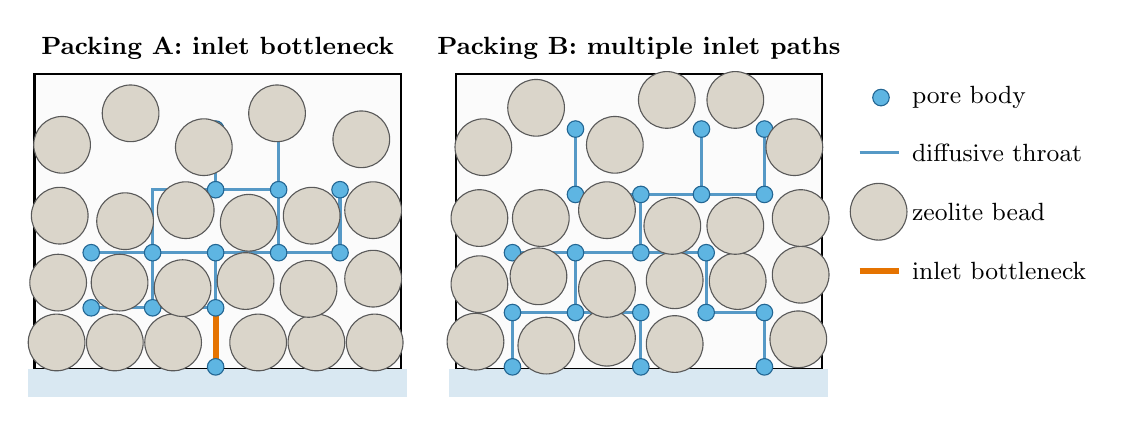
\begin{tikzpicture}[
  	beadS/.style={circle,draw=black!65,fill=zeogray,minimum size=7.2mm,inner sep=0pt},
  	beadM/.style={circle,draw=black!65,fill=zeogray,minimum size=7.2mm,inner sep=0pt},
  	beadL/.style={circle,draw=black!65,fill=zeogray,minimum size=7.2mm,inner sep=0pt},
  	pore/.style={circle,draw=co2blue!80!black,fill=poreblue,minimum size=2.1mm,inner sep=0pt},
  	throat/.style={draw=co2blue!80,line width=1.15pt},
  	bottleneck/.style={draw=orange!90!black,line width=2.2pt},
  	paneltitle/.style={font=\small\bfseries,align=center},
  	note/.style={font=\small,align=left}]

  	% Packing A: one restricted inlet-connected route.
  	\begin{scope}[shift={(0,0)}]
  		\fill[gray!3] (0,0) rectangle (4.65,3.75); \draw[thick] (0,0) rectangle (4.65,3.75);
  		\fill[co2blue!18] (-0.08,-0.35) rectangle (4.73,0);
  		\node[paneltitle] at (2.325,4.08) {Packing A: inlet bottleneck};
  		% The complete connected pore network is blue. It has no direct inlet
  		% connection except through the single orange bottleneck at x=2.30.
  		\draw[throat] (0.72,0.78)--(1.50,0.78)--(1.50,1.48)--(0.72,1.48);
  		\draw[throat] (1.50,0.78)--(2.30,0.78)--(2.30,1.48)--(1.50,1.48);
  		\draw[throat] (2.30,1.48)--(3.10,1.48)--(3.10,2.28)--(2.30,2.28)--(1.50,2.28)--(1.50,1.48);
  		\draw[throat] (3.10,1.48)--(3.88,1.48)--(3.88,2.28);
  		\draw[throat] (2.30,2.28)--(2.30,3.05); \draw[throat] (3.10,2.28)--(3.10,3.05);
  		% The only reservoir-to-network connection and its accessible backbone.
  		\draw[bottleneck] (2.30,0.03)--(2.30,0.78);
  		\draw[throat] (2.30,0.78)--(2.30,1.48)--(3.10,1.48)--(3.10,2.28)--(2.30,2.28)--(2.30,3.05);
  		\foreach \x/\y in {0.72/0.78,1.50/0.78,0.72/1.48,1.50/1.48,3.88/1.48,3.88/2.28,3.10/3.05} \node[pore] at (\x,\y) {};
  		\foreach \x/\y in {2.30/0.03,2.30/0.78,2.30/1.48,3.10/1.48,3.10/2.28,2.30/2.28,2.30/3.05} \node[pore] at (\x,\y) {};
  		% A nearly closed bottom layer: neighbouring beads touch/overlap visually, so
  		% no additional inlet opening can be inferred.
  		\node[beadM] at (0.28,0.34) {}; \node[beadM] at (1.02,0.34) {}; \node[beadM] at (1.76,0.34) {}; \node[beadM] at (2.84,0.34) {}; \node[beadM] at (3.58,0.34) {}; \node[beadM] at (4.32,0.34) {};
  		\node[beadM] at (0.30,1.10) {}; \node[beadM] at (1.08,1.10) {}; \node[beadM] at (1.88,1.03) {}; \node[beadM] at (2.68,1.12) {}; \node[beadM] at (3.48,1.02) {}; \node[beadM] at (4.30,1.15) {};
  		\node[beadM] at (0.32,1.95) {}; \node[beadM] at (1.15,1.88) {}; \node[beadM] at (1.92,2.02) {}; \node[beadM] at (2.72,1.86) {}; \node[beadM] at (3.52,1.95) {}; \node[beadM] at (4.30,2.02) {};
  		\node[beadM] at (0.35,2.85) {}; \node[beadM] at (1.22,3.25) {}; \node[beadM] at (2.15,2.82) {}; \node[beadM] at (3.08,3.25) {}; \node[beadM] at (4.15,2.92) {};
  	\end{scope}

  	% Packing B: several parallel inlet-connected routes.
  	\begin{scope}[shift={(5.35,0)}]
  		\fill[gray!3] (0,0) rectangle (4.65,3.75); \draw[thick] (0,0) rectangle (4.65,3.75);
  		\fill[co2blue!18] (-0.08,-0.35) rectangle (4.73,0);
  		\node[paneltitle] at (2.325,4.08) {Packing B: multiple inlet paths};
  		\draw[throat] (0.72,0.03)--(0.72,0.72)--(1.52,0.72)--(1.52,1.48)--(2.35,1.48)--(2.35,2.22)--(3.12,2.22)--(3.12,3.05);
  		\draw[throat] (2.35,0.03)--(2.35,0.72)--(1.52,0.72);
  		\draw[throat] (3.92,0.03)--(3.92,0.72)--(3.18,0.72)--(3.18,1.48)--(2.35,1.48);
  		\draw[throat] (0.72,1.48)--(1.52,1.48); \draw[throat] (2.35,2.22)--(1.52,2.22)--(1.52,3.05);
  		\draw[throat] (3.12,2.22)--(3.92,2.22)--(3.92,3.05);
  		\foreach \x/\y in {0.72/0.03,0.72/0.72,1.52/0.72,1.52/1.48,2.35/1.48,2.35/2.22,3.12/2.22,3.12/3.05,2.35/0.03,2.35/0.72,3.92/0.03,3.92/0.72,3.18/0.72,3.18/1.48,0.72/1.48,1.52/2.22,1.52/3.05,3.92/2.22,3.92/3.05} \node[pore] at (\x,\y) {};
  		\node[beadS] at (0.25,0.35) {}; \node[beadL] at (1.15,0.30) {}; \node[beadS] at (1.92,0.40) {}; \node[beadM] at (2.78,0.32) {}; \node[beadL] at (4.35,0.38) {};
  		\node[beadL] at (0.30,1.08) {}; \node[beadS] at (1.05,1.18) {}; \node[beadM] at (1.92,1.02) {}; \node[beadL] at (2.78,1.13) {}; \node[beadS] at (3.58,1.12) {}; \node[beadM] at (4.38,1.20) {};
  		\node[beadS] at (0.30,1.92) {}; \node[beadM] at (1.08,1.92) {}; \node[beadL] at (1.92,2.02) {}; \node[beadS] at (2.75,1.82) {}; \node[beadM] at (3.55,1.82) {}; \node[beadL] at (4.38,1.92) {};
  		\node[beadM] at (0.35,2.82) {}; \node[beadL] at (1.02,3.32) {}; \node[beadS] at (2.02,2.85) {}; \node[beadM] at (2.68,3.42) {}; \node[beadL] at (3.55,3.42) {}; \node[beadS] at (4.30,2.82) {};
  	\end{scope}

  	\node[pore] at (10.75,3.45) {}; \node[note,anchor=west] at (11.02,3.45) {pore body};
  	\draw[throat] (10.48,2.75)--(10.98,2.75); \node[note,anchor=west] at (11.02,2.75) {diffusive throat};
  	\node[beadM] at (10.72,2.0) {}; \node[note,anchor=west] at (11.02,2.0) {zeolite bead};
  	\draw[bottleneck] (10.48,1.25)--(10.98,1.25); \node[note,anchor=west] at (11.02,1.25) {inlet bottleneck};
  \end{tikzpicture}%
  \vfill\small Same beads and similar porosity; different numbers and conductances of inlet-connected paths.
  \note{
    This schematic introduces the central problem. The two beds contain the
    same monodisperse beads and can have almost the same total porosity. Their
    inlet-connected paths can nevertheless differ strongly. Packing A
    illustrates a network reached through one restrictive inlet bottleneck.
    Packing B illustrates several paths that connect the reservoir to the bed
    interior.

    The blue lines show only simplified inlet-connected paths, not every throat
    in a real extracted network. The sketches are therefore hypotheses rather
    than simulation results. They motivate our research question: can a
    quantitative pore-accessibility measure predict transient bed-scale
    transport better than bulk porosity alone?
  }
\end{frame}

\begin{frame}{Why zeolite 13X and what does the study isolate?}
  \vspace*{-0.45cm}
  \begin{FlexRow}{0.59\textheight}
    \Col{0.48}{
      \footnotesize
      \hi{Why zeolite 13X?}
      \begin{itemize}
        \item established benchmark sorbent for CO$_2$
        \item strong equilibrium uptake at low partial pressure
        \item commercial millimetre-scale beads form random beds
      \end{itemize}
      \vspace{0.25cm}
      \hi{Controlled model problem}
      \begin{itemize}
        \item dry, isothermal, stagnant gas
        \item CO$_2$ enters from a reservoir below the bed
        \item pore-network model resolves throat diffusion and bead adsorption
        \item no imposed flow; no CFD
      \end{itemize}}
    \Col{0.48}{
      \question{How strongly does random void connectivity change access to the adsorbent?}
      \vspace{0.30cm}
      \centering
      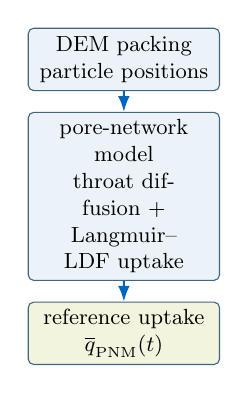
\begin{tikzpicture}[node distance=3mm,scale=.88,transform shape]
        \node[box] (dem) {DEM packing\\particle positions};
        \node[box,below=of dem] (pnm) {pore-network model\\throat diffusion +\\Langmuir--LDF uptake};
        \node[box,below=of pnm,fill=tumgreen!13] (resp) {reference uptake\\$\overline q_{\rm PNM}(t)$};
        \draw[arr] (dem)--(pnm);\draw[arr] (pnm)--(resp);
      \end{tikzpicture}}
  \end{FlexRow}
  \note{
    We use zeolite 13X because it is a well-established benchmark sorbent for
    CO$_2$. It has strong equilibrium uptake at low partial pressure and is
    available as millimetre-scale beads that naturally form random beds.

    The study deliberately isolates one mechanism. The gas is dry,
    isothermal and stagnant. CO$_2$ enters from a reservoir below the bed. We
    do not impose a gas flow and we do not solve CFD. We do, however, model the
    pore space explicitly. Starting from the DEM particle positions, the
    pore-network model resolves diffusion through the throats and couples it to
    Langmuir equilibrium and finite-rate adsorption in the beads. Its principal
    reference output is the mean network uptake curve,
    $\overline q_{\rm PNM}(t)$.
  }
\end{frame}

\section[Model scope]{Model scope and physical mechanisms}
\begin{frame}{}
\vfill
{\large\color{tumgray}Section 2 of 5}\par\vspace{0.4cm}
{\LARGE\color{tumblue}\textbf{Model scope and physical mechanisms}}\par\vspace{0.5cm}
{\large From particle arrangement to diffusion and adsorption}
\vfill
\note{From particle arrangement to diffusion and adsorption.}
\end{frame}

\begin{frame}{Twenty beds isolate variability caused by random arrangement}
  \begin{FlexRow}{0.57\textheight}
    \Col{0.43}{
      \begin{tabular}{ll}\toprule
      Quantity & Fixed value\\\midrule
      beads per bed & 1850\\
      bead diameter & 1.6 mm\\
      tube diameter & 16 mm\\
      $D_{\rm tube}/d_p$ & 10\\
      temperature & 298.15 K\\
      inlet $c_{\rm CO_2}$ & 6.05 mol m$^{-3}$\\
      simulation time & 5000 s\\\bottomrule
      \end{tabular}}
    \Col{0.53}{
      \hi{Only the DEM insertion seed changed}
      \begin{itemize}
        \item Delaunay--Voronoi networks were built directly from particle coordinates
        \item all networks were connected and spanning
        \item quasi-uniform Sobol sampling allocated pore volumes without a voxel grid
        \item transient and 1D models passed mass-balance checks
      \end{itemize}}
  \end{FlexRow}

  \vspace*{0.5cm}
  \result{The ensemble tests arrangement effects under otherwise identical conditions.}
  \note{
    We generated twenty independent beds. Every listed physical and numerical
    condition remains fixed, including the number and diameter of the beads,
    tube diameter, temperature, inlet concentration and simulation duration.
    Only the DEM insertion seed changes. Differences between the cases can
    therefore be attributed to the random arrangement rather than to changed
    operating conditions.

    We construct a Delaunay--Voronoi pore network directly from the particle
    coordinates. Sobol sampling means a deterministic, low-discrepancy set of
    quasi-uniform points. We use these points only to allocate the analytically
    calculated void volume among pore bodies. They do not create the network
    connectivity, and no voxel grid is required. All twenty networks span the
    bed and pass the mass-balance checks.
  }
\end{frame}

\begin{frame}{Pore-network geometry and throat diffusion}
  \begin{columns}[T,onlytextwidth]
    \column{0.46\textwidth}
      \hi{Network construction}
      \footnotesize
      \begin{itemize}
        \item four bead centres define a Delaunay tetrahedron; its circumcentre is a pore body
        \item tetrahedra sharing a triangular face are joined by a throat
        \item topology comes from particle coordinates, not voxels
      \end{itemize}
      \vspace{0.12cm}
      A low-discrepancy Sobol sample of $2^{22}$ points allocates the analytically
      calculated void volume to pore bodies; it does not define connectivity.
    \column{0.50\textwidth}
      \hi{Diffusion through throat $i$--$j$}
      \[
        G_{ij}=D_m\frac{A_{ij}}{L_{ij}},\qquad
        \dot n_{ij}=G_{ij}(c_j-c_i).
      \]
      \footnotesize
      $L_{ij}=\lVert\mathbf{x}_j-\mathbf{x}_i\rVert$ is the pore-centre distance.
      The irregular opening between three beads is approximated by an equivalent
      circular area
      \[
        A_{ij}=\pi r_{ij}^{2},
      \]
      where $r_{ij}$ is the clearance of the shared Delaunay face.
  \end{columns}
  \vspace{0.16cm}
  \result{The circular throat area is a geometric modelling assumption; $G_{ij}$ has units of m$^3$ s$^{-1}$.}
  \note{
    Four neighbouring bead centres define a Delaunay tetrahedron, and its
    circumcentre becomes a pore body. Two tetrahedra sharing a triangular face
    create two neighbouring pores connected by a throat. The indices $i$ and
    $j$ therefore refer to adjacent pore bodies.

    Diffusion through that throat follows
    $G_{ij}=D_m A_{ij}/L_{ij}$. Here $D_m$ has units of square metres per
    second, $A_{ij}$ has units of square metres and $L_{ij}$ has units of
    metres. Thus, $G_{ij}$ has units of cubic metres per second. Multiplying it
    by the concentration difference gives the molar flow rate through the
    throat. The actual opening is irregular. We approximate it by a circular
    area $A_{ij}=\pi r_{ij}^2$. This equivalent circular area is an explicit
    geometric assumption of the model.
  }
\end{frame}

\begin{frame}{Langmuir equilibrium and bead uptake}
  \begin{columns}[T,onlytextwidth]
    \column{0.52\textwidth}
      \hi{Local equilibrium loading}
      \[
        p_k=c_kRT,\qquad
        q_k^*=\frac{q_s\,b\,p_k}{1+b\,p_k}.
      \]
      \hi{Finite-rate uptake}
      \[
        \frac{dq_k}{dt}=k_{\rm LDF}\,(q_k^*-q_k).
      \]
      \small
      $q_s$ is the maximum CO$_2$ loading [mol/kg adsorbent].
      $b$ is the Langmuir affinity,
      $p_k$ is the local CO$_2$ partial pressure, and $q_k^*$ is the
      corresponding equilibrium loading. The product $b\,p_k$ is dimensionless.
    \column{0.44\textwidth}
      \hi{Meaning of the rate equation}
      \small
      \begin{itemize}
        \item $q_k$ is the current loading of bead $k$
        \item $k_{\rm LDF}$ controls how quickly $q_k$ approaches $q_k^*$
        \item gas removed from adjacent pores is added to the bead
      \end{itemize}
      \vspace{0.18cm}
      \hi{Pore-network outputs}
      \begin{itemize}
        \item pore concentrations $c_i(t)$
        \item particle loadings $q_k(t)$
        \item mean uptake $\overline q_{\rm PNM}(t)$
      \end{itemize}
  \end{columns}
  \result{The coupled diffusion--adsorption calculation conserves the total amount of CO$_2$.}
  \note{
    Diffusion supplies a local gas concentration $c_k$ around bead $k$. We
    convert it to partial pressure through $p_k=c_kRT$. The Langmuir equation
    then gives the equilibrium loading $q_k^*$. The parameter $q_s$ is the
    saturation loading and $b$ is the Langmuir affinity. Because $b$ has units
    of inverse pressure, the product $b p_k$ is dimensionless.

    The actual particle loading $q_k$ does not jump immediately to equilibrium.
    The linear-driving-force equation describes how it approaches $q_k^*$,
    with $k_{\rm LDF}$ setting the uptake rate. Gas removed from the pores is
    added to the particles, so the coupled calculation conserves CO$_2$. The
    detailed outputs include every pore concentration $c_i(t)$ and every bead
    loading $q_k(t)$. Averaging the bead inventory gives the reference uptake
    curve $\overline q_{\rm PNM}(t)$.
  }
\end{frame}

\section[Methods]{Numerical methods and diffusivity prediction}
\begin{frame}{}
\vfill
{\large\color{tumgray}Section 3 of 5}\par\vspace{0.4cm}
{\LARGE\color{tumblue}\textbf{Numerical methods and diffusivity prediction}}\par\vspace{0.5cm}
{\large How we calculate accessibility and calibrate the reduced model}
\vfill
\note{How we calculate accessibility and calibrate the reduced model.}
\end{frame}

\begin{frame}{Development and later use are two different workflows}
  \centering
  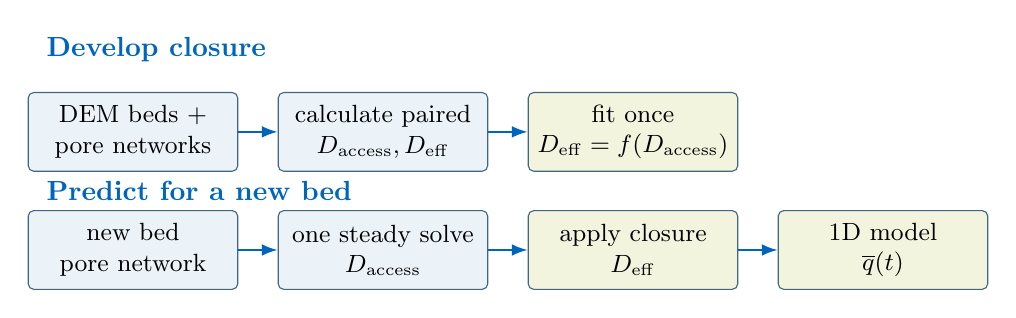
\begin{tikzpicture}[node distance=5mm and 5mm,
    flowbox/.style={box,text width=2.45cm,minimum height=10mm}]
    \node[font=\bfseries,text=tumblue,anchor=west] at (-1.22,1.05) {Develop closure};
    \node[flowbox] (beds) {DEM beds +\\pore networks};
    \node[flowbox,right=of beds] (pair) {calculate paired\\$D_{\rm access},D_{\rm eff}$};
    \node[flowbox,right=of pair,fill=tumgreen!13] (close) {fit once\\$D_{\rm eff}=f(D_{\rm access})$};
    \draw[arr] (beds)--(pair);\draw[arr] (pair)--(close);
    \node[font=\bfseries,text=tumblue,anchor=west] at (-1.22,-0.75) {Predict for a new bed};
    \node[flowbox] (new) at (0,-1.5) {new bed\\pore network};
    \node[flowbox,right=of new] (steady) {one steady solve\\$D_{\rm access}$};
    \node[flowbox,right=of steady,fill=tumgreen!13] (pred) {apply closure\\$D_{\rm eff}$};
    \node[flowbox,right=of pred,fill=tumgreen!13] (uptake) {1D model\\$\overline q(t)$};
    \draw[arr] (new)--(steady);\draw[arr] (steady)--(pred);\draw[arr] (pred)--(uptake);
  \end{tikzpicture}

  \vspace{0.45cm}
  \result{For a new bed, the transient pore-network adsorption model is no longer required.}
  \note{
    This slide separates development from later prediction. During development,
    we run the full transient pore-network adsorption model for each training
    bed. From its uptake curve, we fit one effective diffusivity,
    $D_{\rm eff}$. Independently, one steady network solve gives the
    accessibility diffusivity, $D_{\rm access}$. The paired values across the
    beds allow us to fit the closure
    $D_{\rm eff}=f(D_{\rm access})$.

    For a new packing, the lower workflow applies. We still extract its pore
    network, but we perform only the inexpensive steady accessibility solve.
    The closure predicts $D_{\rm eff}$, and the 1D model then predicts the
    complete uptake curve. The expensive transient pore-network adsorption
    calculation belongs to development and validation, not to routine use.
  }
\end{frame}

\begin{frame}{The homogeneous 1D uptake model}
  \begin{columns}[T,onlytextwidth]
    \column{0.55\textwidth}
      \hi{Axial diffusion and adsorption}
      \small
      \[
        \varepsilon_b\frac{\partial c}{\partial t}
        =D\frac{\partial^2c}{\partial z^2}
        -(1-\varepsilon_b)\rho_p\frac{\partial q}{\partial t},
      \]
      \[
        \frac{\partial q}{\partial t}
        =k_{\rm LDF}\,[q^*(c)-q].
      \]
      For each trial $D$, solve both equations together for $c(z,t)$ and
      $q(z,t)$ in 100 cells, with prescribed initial and boundary conditions.
    \column{0.41\textwidth}
      \hi{Quantity compared with the network}
      \[
        \overline q_{\rm 1D}(t;D)
        =\frac{1}{H}\int_0^H q(z,t;D)\,dz.
      \]
      \small
      The 1D model uses the same bed height, porosity, inlet condition,
      Langmuir parameters, LDF coefficient and initial state as the pore network.
      Only $D$ changes during fitting.
  \end{columns}
  \vspace{0.18cm}
  \result{For every trial $D$, the 1D solver produces a complete mean uptake curve.}
  \note{
    The reduced model replaces the irregular pore network by one axial
    coordinate. It solves coupled diffusion and adsorption in one hundred
    cells. The local outputs are the gas concentration $c(z,t)$ and loading
    $q(z,t)$. Their spatial average gives
    $\overline q_{\rm 1D}(t;D)$, the mean uptake predicted by the 1D model.

    The bed height, porosity, inlet condition, Langmuir parameters, LDF
    coefficient and initial state remain identical to those in the pore-network
    calculation. Only the diffusivity $D$ changes. For any selected value of
    $D$, the solver must integrate the complete transient problem and return a
    complete uptake curve. This is why we call it a trial diffusivity at this
    stage. We do not yet know which value best represents the network.
  }
\end{frame}

\begin{frame}{$D_{\rm access}$ and $D_{\rm eff}$ answer different questions}
  \begin{columns}[T,onlytextwidth]
    \column{0.47\textwidth}
      \hi{$D_{\rm access}$: geometric accessibility}
      \footnotesize
      \begin{itemize}
        \item fix concentration at inlet and interior plane
        \item solve one steady, linear diffusion problem
        \item no adsorption and no time integration
      \end{itemize}
      \[
        D_{\rm access}=\frac{G_{\rm access}H}{A_{\rm tube}}.
      \]
      $G_{\rm access}$ is total steady flux per concentration difference.
      $H$ is bed height; $A_{\rm tube}$ is tube area.
    \column{0.47\textwidth}
      \hi{$D_{\rm eff}$: transient reduced-model coefficient}
      \footnotesize
      \begin{itemize}
        \item full transient network gives $\overline q_{\rm PNM}(t)$
        \item repeated 1D solves give $\overline q_{\rm 1D}(t;D)$
      \end{itemize}
      Define the curve residual
      \[
        e_m(D)=\overline q_{\rm 1D}(t_m;D)-\overline q_{\rm PNM}(t_m).
      \]
      \vspace{-0.20cm}
      \[
        \begin{aligned}
        \mathrm{NRMSE}(D)&=
          \frac{\sqrt{\sum_m w_m e_m(D)^2}}{\overline q_{\rm PNM}(t_f)},\\[-1mm]
        D_{\rm eff}&=\arg\min_D\mathrm{NRMSE}(D).
        \end{aligned}
      \]
      The trapezoidal weights $w_m$ account for unequal time spacing and satisfy
      $\sum_m w_m=1$.
  \end{columns}
  \vspace{0.10cm}
  \begin{beamercolorbox}[rounded=true,sep=0.35em]{block body}
    \centering\small\bfseries\color{tumdark}
    $D_{\rm access}$ is cheap because it avoids adsorption dynamics and optimization.
  \end{beamercolorbox}
  \note{
    These two quantities answer different questions. To calculate
    $D_{\rm access}$, we prescribe concentrations at the inlet and at an
    interior plane and solve one steady linear diffusion problem. Steady here
    means that we directly solve the time-independent balance. We do not run a
    transient simulation and wait for physical steady state. The result is the
    total conductance $G_{\rm access}$ between the two boundaries. Multiplying
    it by bed height and dividing by tube area expresses it in diffusivity
    units.

    $D_{\rm eff}$ is different. It is the coefficient required by the reduced
    1D transient model. The network first supplies
    $\overline q_{\rm PNM}(t)$. We choose a trial $D$, solve the 1D transient
    model and obtain $\overline q_{\rm 1D}(t;D)$. The optimizer then changes
    $D$ and repeats the 1D solve. At every saved time, $e_m(D)$ is the
    difference between the 1D and network uptake. NRMSE combines these errors
    over the full curve. Squaring prevents positive and negative errors from
    cancelling, the square root restores loading units, and division by the
    final network loading makes the result dimensionless. The time weights
    account for unequal intervals. The value that minimizes NRMSE is called
    $D_{\rm eff}$. This optimization explains why obtaining $D_{\rm eff}$ is
    more expensive than calculating $D_{\rm access}$.
  }
\end{frame}

\begin{frame}{Why use an interior plane?}
  \begin{FlexRow}{0.61\textheight}
    \Col{0.50}{\centering
      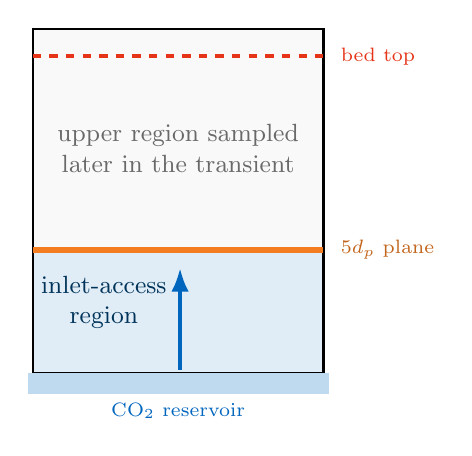
\begin{tikzpicture}[x=0.82cm,y=0.78cm]
        \fill[tumblue!12] (0,0) rectangle (4.5,2.0);
        \fill[gray!5] (0,2.0) rectangle (4.5,5.6);
        \draw[thick] (0,0) rectangle (4.5,5.6);
        \fill[tumblue!25] (-.08,-.35) rectangle (4.58,0);
        \node[font=\scriptsize,tumblue] at (2.25,-.62) {CO$_2$ reservoir};
        \draw[-{Latex},very thick,tumblue] (2.28,.05)--(2.28,1.70);
        \draw[tumorange,line width=2pt] (0,2.0)--(4.5,2.0);
        \node[anchor=west,font=\scriptsize,tumorange!80!black] at (4.62,2.0) {$5d_p$ plane};
        \draw[tumred,dashed,line width=1.4pt] (0,5.15)--(4.5,5.15);
        \node[anchor=west,font=\scriptsize,tumred] at (4.62,5.15) {bed top};
        \node[align=center,font=\small,tumdark] at (1.1,1.15) {inlet-access\\region};
        \node[align=center,font=\small,tumgray] at (2.25,3.65) {upper region sampled\\later in the transient};
      \end{tikzpicture}}
    \Col{0.46}{
      \small
      \hi{A plane at $5d_p$ includes}
      \begin{itemize}
        \item the inlet openings
        \item second-layer and deeper bottlenecks
        \item parallel paths connecting inlet to the plane
      \end{itemize}
      \vspace{0.25cm}
      \hi{The bed top answers a different question}

      \vspace*{-0.05cm}
      \begin{itemize}
        \item measure conductance through the entire bed
        \item include upper bottlenecks not sampled early
      \end{itemize}}
  \end{FlexRow}
  \note{
    The accessibility calculation connects the inlet to an interior plane at a
    selected depth. It includes every connected path and every bottleneck
    between these two boundaries. Therefore, a bottleneck in the second layer
    or any deeper layer below the plane directly reduces
    $G_{\rm access}$.

    We use an interior plane because the descriptor targets access from the
    inlet into the region sampled during the earlier part of adsorption. A
    plane at the bed top would instead measure steady conductance through the
    complete bed. It would include upper restrictions that affect the response
    mainly later in the transient. This does not mean that upper bottlenecks are
    physically unimportant. It means that whole-bed conductance answers a
    different question from inlet accessibility. The appropriate depth must
    therefore be checked rather than assumed.
  }
\end{frame}

\begin{frame}{Why not predict uptake directly from $G_{\rm access}$?}
  \begin{columns}[T,onlytextwidth]
    \column{0.46\textwidth}
      \hi{Direct endpoint relation}
      \[
        G_{\rm access}\longrightarrow \overline q(5000\,{\rm s})
      \]
      \small
      \begin{itemize}
        \item strong correlation: $\rho_s=0.968$
        \item ranks beds or predicts one endpoint
        \item valid at the selected time and conditions
      \end{itemize}
    \column{0.49\textwidth}
      \hi{Transport closure}
      \[
        G_{\rm access}\longrightarrow D_{\rm access}
        \longrightarrow D_{\rm eff}\longrightarrow \overline q(t)
      \]
      \small
      \begin{itemize}
        \item generates the complete uptake curve
        \item retains conservative 1D transport
        \item gives axial $c(z,t)$ and $q(z,t)$ profiles
      \end{itemize}
  \end{columns}
  \vspace{0.28cm}
  \result{If only uptake at 5000 s is needed, $G_{\rm access}$ is sufficient; $D_{\rm eff}$ is needed for a reusable transient model.}
  \note{
    Accessibility conductance correlates very strongly with uptake at 5000
    seconds. If our only task were to rank beds or estimate this one endpoint
    under the same conditions, we could use $G_{\rm access}$ directly.

    Our intended reduced model asks for more. We want the complete uptake curve
    and the axial concentration and loading profiles. The 1D conservation
    equations require a transport coefficient, which is $D_{\rm eff}$.
    Furthermore, $D_{\rm access}$ should not simply be inserted as
    $D_{\rm eff}$ because the strict proportional model performs substantially
    worse than the fitted power-law closure. The sequence is therefore:
    calculate $D_{\rm access}$ cheaply, predict $D_{\rm eff}$ through the
    closure, and use $D_{\rm eff}$ in the transient 1D model.
  }
\end{frame}

\begin{frame}{Diffusivity optimization and closure calibration}
\begin{columns}[T,onlytextwidth]
\column{0.49\textwidth}
\hi{Fit one diffusivity per bed}
\small
\begin{enumerate}
\item Choose a trial $D$ within prescribed bounds.
\item Solve the coupled 1D equations for $c(z,t)$ and $q(z,t)$.
\item Compare mean uptake with the network using time-weighted NRMSE.
\item Use previous errors to select the next $D$ and repeat (optimization).
\end{enumerate}
\column{0.47\textwidth}
\hi{Learn the relationship across beds}
\small
\begin{itemize}
\item Pair each fitted $D_{\rm eff}$ with its geometry-based $D_{\rm access}$.
\item Fit the closure $D_{\rm eff}=f(D_{\rm access})$ on the training beds.
\item Leave one bed out to assess diffusivity prediction.
\end{itemize}
\medskip
The bounded search operates in $\log_{10}D$ and starts deterministically.
\end{columns}
\vspace{0.2cm}
\result{Per-bed optimization supplies the targets for closure calibration.}
\note{There are two fitting tasks. First, for each bed, optimize one diffusivity to match its network uptake curve. Each trial restarts the coupled transient model from the prescribed initial state. Then learn a relationship between these fitted targets and accessibility across beds. In leave-one-bed-out evaluation, fit that relationship on nineteen beds and predict the twentieth. This is internal validation within the current ensemble.}
\end{frame}

\section[Results]{Results and robustness}
\begin{frame}{}
\vfill
{\large\color{tumgray}Section 4 of 5}\par\vspace{0.4cm}
{\LARGE\color{tumblue}\textbf{Results and robustness}}\par\vspace{0.5cm}
{\large Uptake variability, predictive closure and depth sensitivity}
\vfill
\note{Uptake variability, predictive closure and depth sensitivity.}
\end{frame}

\begin{frame}{The twenty beds have nearly equal bulk porosity}
  \begin{columns}[c,onlytextwidth]
    \column{0.65\textwidth}
    \centering
    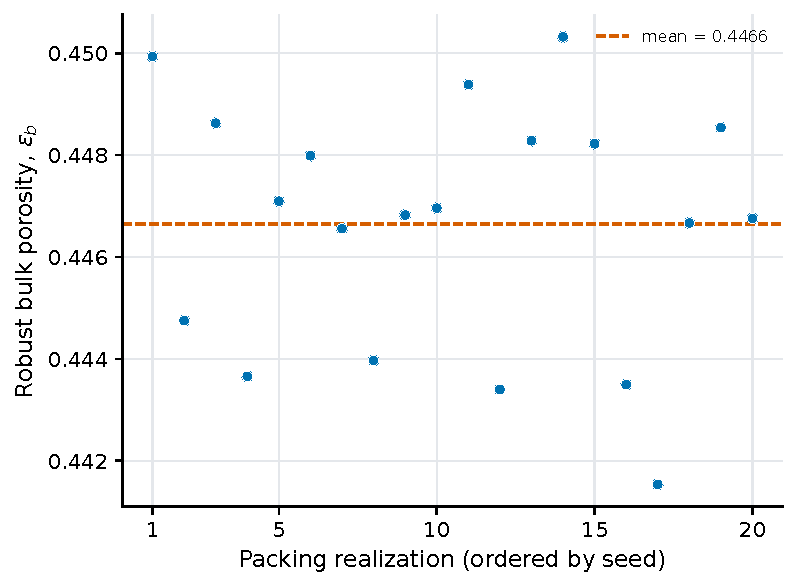
\includegraphics[width=\linewidth,height=0.69\textheight,keepaspectratio]{figures/fig_porosity_variability.pdf}
    \column{0.32\textwidth}
    \small
    \hi{Controlled ensemble}
\begin{itemize}
\item same bead count and diameter
\item same tube geometry
\item only the insertion seed changes
\end{itemize}
\medskip
CV: coefficient of variation\\[0.15cm]
$\mathrm{CV}_{\varepsilon}=s_{\varepsilon}/\overline{\varepsilon}$\\[0.15cm]
$s_{\varepsilon}$: standard deviation\\
$\overline{\varepsilon}$: mean porosity
  \end{columns}
  \vspace{0.12cm}
  {\small\result{Bulk-porosity CV: $0.55\%$.}}
  \note{The mean bulk porosity is approximately 0.44665. Divide the sample standard deviation by this mean to obtain the coefficient of variation, 0.55 percent. The horizontal axis orders beds by their insertion seed. The small spread establishes the controlled comparison.}
\end{frame}

\begin{frame}{Similar porosity still produces different uptake curves}
  \begin{columns}[c,onlytextwidth]
    \column{0.65\textwidth}
    \centering
    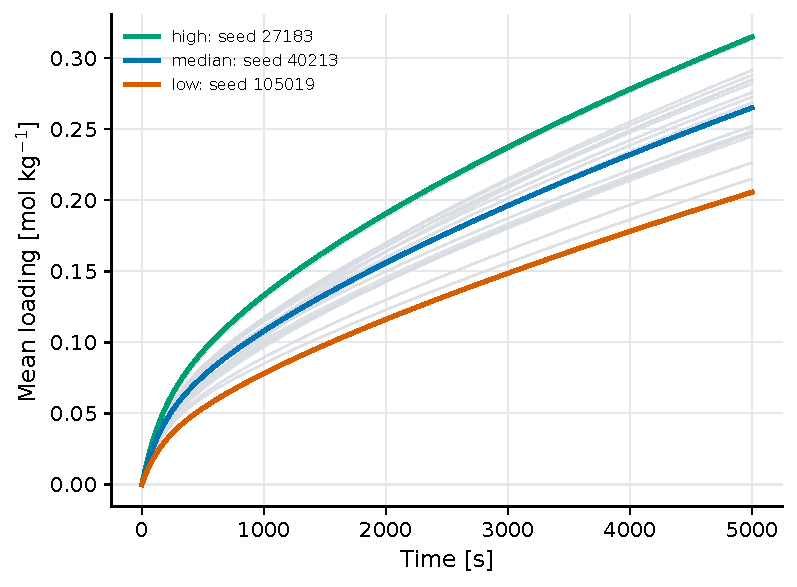
\includegraphics[width=\linewidth,height=0.69\textheight,keepaspectratio]{figures/fig_uptake_curves.pdf}
    \column{0.32\textwidth}
    \small
    \hi{Network reference}
\begin{itemize}
\item all twenty uptake curves
\item highlighted beds span low, median and high final uptake
\item identical adsorption parameters
\end{itemize}
  \end{columns}
  \vspace{0.12cm}
  {\small\result{At 5000 s: $0.206$--$0.315$ mol kg$^{-1}$, with an uptake CV of $11.0\%$.}}
  \note{The pale curves show the full ensemble. Orange, blue and green identify low, median and high final uptake. These representative beds are selected by final uptake, not by accessibility. The uptake varies much more strongly than porosity.}
\end{frame}

\begin{frame}{Bulk porosity alone does not explain final uptake}
  \begin{columns}[c,onlytextwidth]
    \column{0.65\textwidth}
    \centering
    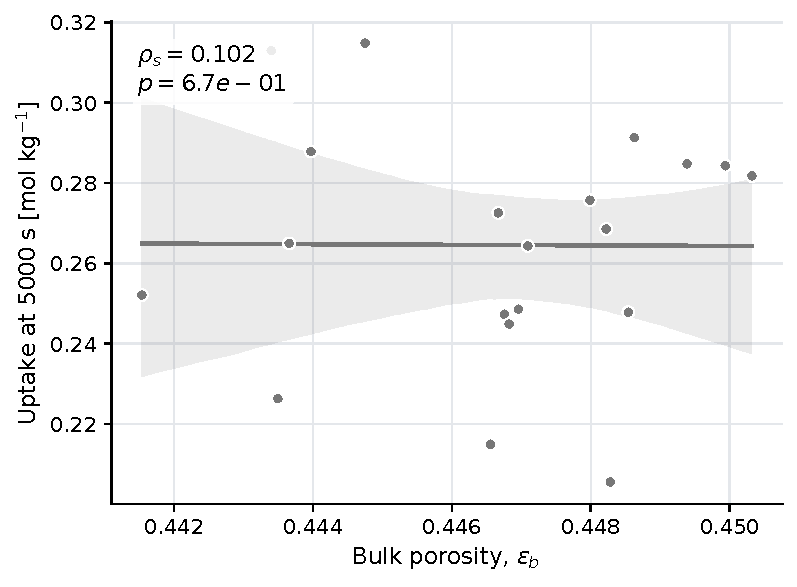
\includegraphics[width=\linewidth,height=0.69\textheight,keepaspectratio]{figures/fig_porosity_uptake.pdf}
    \column{0.32\textwidth}
    \small
    \hi{Porosity baseline}
\begin{itemize}
\item each point represents one bed
\item weak rank association
\item wide uncertainty around the fitted relationship
\end{itemize}
  \end{columns}
  \vspace{0.12cm}
  {\small\result{Void volume alone does not describe access to the adsorbent.}}
  \note{The plot compares bulk porosity with mean loading at 5000 seconds. Spearman correlation is approximately 0.102. The shaded band is pointwise bootstrap uncertainty in the fitted relationship, not a prediction interval for a new bed.}
\end{frame}

\begin{frame}{Accessibility explains differences in final uptake}
  \begin{columns}[c,onlytextwidth]
    \column{0.65\textwidth}
    \centering
    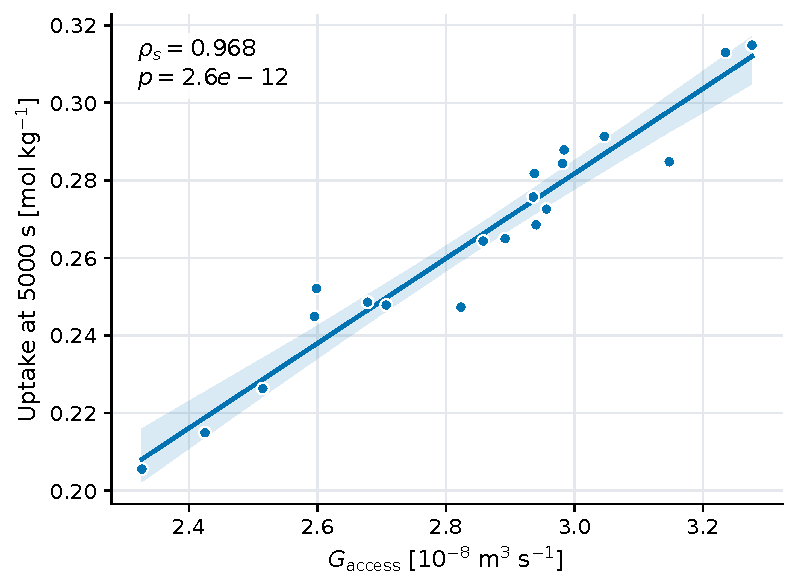
\includegraphics[width=\linewidth,height=0.69\textheight,keepaspectratio]{figures/fig_accessibility_uptake.pdf}
    \column{0.32\textwidth}
    \small
    \hi{Steady network descriptor}
\begin{itemize}
\item $G_{\rm access}$ measures inlet-to-interior conductance
\item greater conductance accompanies greater uptake
\end{itemize}
\medskip
Spearman $\rho_s=0.968$.
  \end{columns}
  \vspace{0.12cm}
  {\small\result{Inlet-connected pathways explain variability that porosity misses.}}
  \note{We calculate accessibility using a steady diffusion problem without adsorption. The Spearman coefficient is 0.968. More accessible beds generally have greater uptake. This is a within-ensemble association. The shaded band represents uncertainty in the fitted relationship.}
\end{frame}

\begin{frame}{Greater accessibility reduces particle underutilization}
  \begin{columns}[c,onlytextwidth]
    \column{0.65\textwidth}
    \centering
    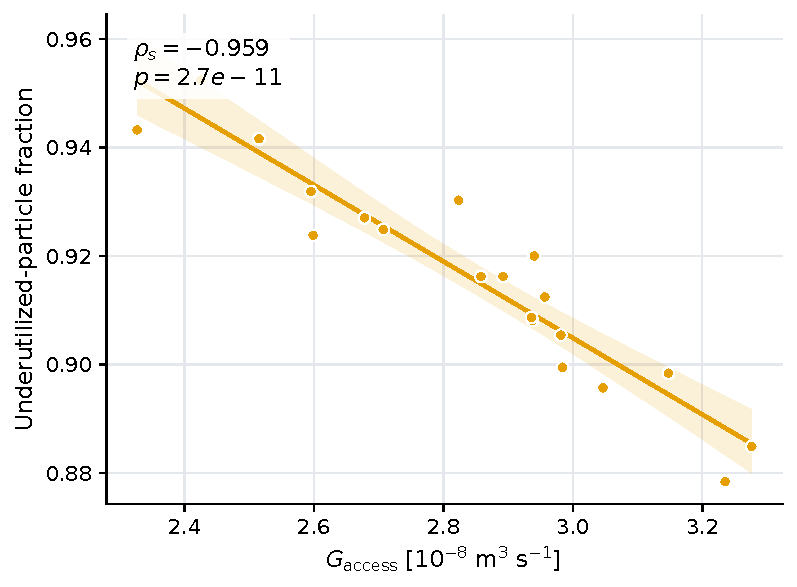
\includegraphics[width=\linewidth,height=0.69\textheight,keepaspectratio]{figures/fig_accessibility_utilization.pdf}
    \column{0.32\textwidth}
    \small
    \hi{Underutilized fraction}
\[
 f_{\rm under}=\frac{1}{N_p}\sum_{k=1}^{N_p} I_k.
\]
$I_k=1$ when
\[
 q_k(t_f)<0.5q^*(p_{\rm inlet}).
\]
$t_f=5000$ s.
\medskip
\par The indicator equals one for a particle below half the inlet-equilibrium loading.
  \end{columns}
  \vspace{0.12cm}
  {\small\result{Higher $G_{\rm access}$ accompanies fewer underutilized particles.}}
  \note{For each bead we compare its final loading with half the equilibrium loading at the inlet pressure. The indicator is one below this threshold and zero otherwise. Averaging over particles gives the plotted fraction. This is a threshold-based utilization measure, not the fraction of completely inaccessible particles.}
\end{frame}

\begin{frame}{One fitted $D_{\rm eff}$ reproduces each uptake curve}
  \begin{columns}[c,onlytextwidth]
    \column{0.65\textwidth}
    \centering
    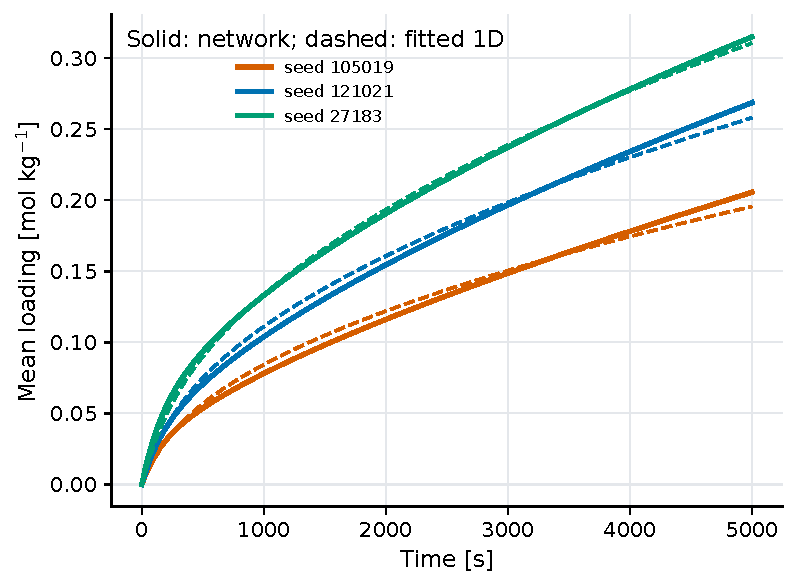
\includegraphics[width=\linewidth,height=0.69\textheight,keepaspectratio]{figures/fig_homogeneous_uptake.pdf}
    \column{0.32\textwidth}
    \small
    \hi{Per-bed optimization}
\begin{enumerate}
\item solve the 1D model for a trial $D$
\item evaluate time-weighted NRMSE against the network curve
\item use previous errors to select the next $D$ and repeat (optimization)
\end{enumerate}
\medskip
Solid: network.\\Dashed: fitted 1D model.
  \end{columns}
  \vspace{0.12cm}
  {\small\result{Across twenty beds, the mean fitted-curve NRMSE is $1.58\%$.}}
  \note{For each bed, the transient pore-network calculation provides a reference uptake curve. We repeatedly solve the 1D model with trial diffusivities and minimize the time-weighted normalized root-mean-square error. The bounded optimizer searches in $\log_{10}D$. Its initial trial follows from the prescribed bounds, without random sampling. Previous objective values guide subsequent trials until the search meets its tolerance. Each trial solves both coupled equations from the same initial state. The optimized diffusivity is $D_{\rm eff}$. This figure shows per-bed fits, not predictions for unseen beds. The mean error is 1.58 percent.}
\end{frame}

\begin{frame}{Residuals show the remaining reduction error}
  \begin{columns}[c,onlytextwidth]
    \column{0.65\textwidth}
    \centering
    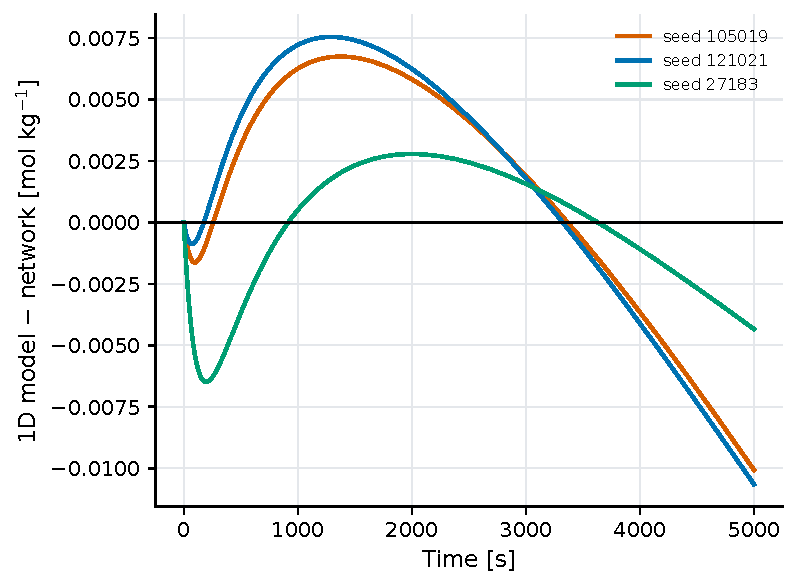
\includegraphics[width=\linewidth,height=0.69\textheight,keepaspectratio]{figures/fig_homogeneous_residuals.pdf}
    \column{0.32\textwidth}
    \small
    \hi{Curve residual}
\[
 e(t)=\overline q_{\rm 1D}(t)-\overline q_{\rm PNM}(t).
\]
\begin{itemize}
\item positive: excess predicted uptake
\item negative: insufficient predicted uptake
\end{itemize}
  \end{columns}
  \vspace{0.12cm}
  {\small\result{Time-weighted NRMSE across all beds: $0.84$--$2.46\%$.}}
  \note{The same three representative beds appear here. The residual is the 1D mean loading minus the network mean loading. Its sign changes over time, showing that one coefficient cannot reproduce every detail. NRMSE summarizes the full residual curve using trapezoidal time weights and normalizes by final network loading.}
\end{frame}

\begin{frame}{A positive power law relates accessibility to diffusivity}
  \begin{columns}[c,onlytextwidth]
    \column{0.65\textwidth}
    \centering
    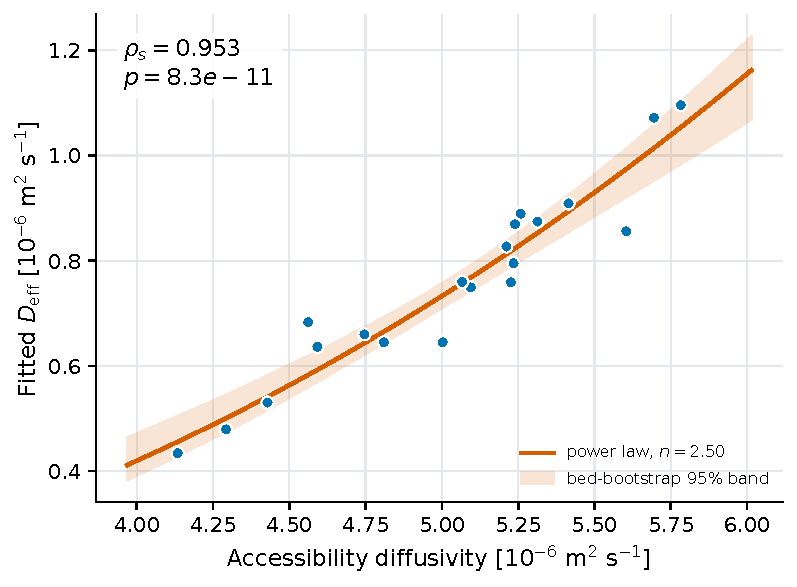
\includegraphics[width=\linewidth,height=0.69\textheight,keepaspectratio]{figures/fig_closure_power_law.pdf}
    \column{0.32\textwidth}
    \small
    \hi{Selected closure}
\[
 \frac{D_{\rm eff}}{D_m}=C\left(\frac{D_{\rm access}}{D_m}\right)^n.
\]
\[
 D_{\rm access}=\frac{G_{\rm access}H}{A_{\rm tube}}.
\]
\medskip
The shaded band shows bootstrap uncertainty in the fitted relationship.
  \end{columns}
  \vspace{0.12cm}
  {\small\result{The fitted exponent is $n\approx2.50$ for this ensemble.}}
  \note{Each bed supplies a geometrically calculated accessibility diffusivity and a diffusivity fitted to its transient response. The power law relates them. This plot shows the fit to the complete ensemble. The band is pointwise bootstrap uncertainty in the relationship, not an individual-bed prediction interval. The exponent is specific to the studied conditions.}
\end{frame}

\begin{frame}{The closure predicts diffusivity for a withheld bed}
  \begin{columns}[c,onlytextwidth]
    \column{0.65\textwidth}
    \centering
    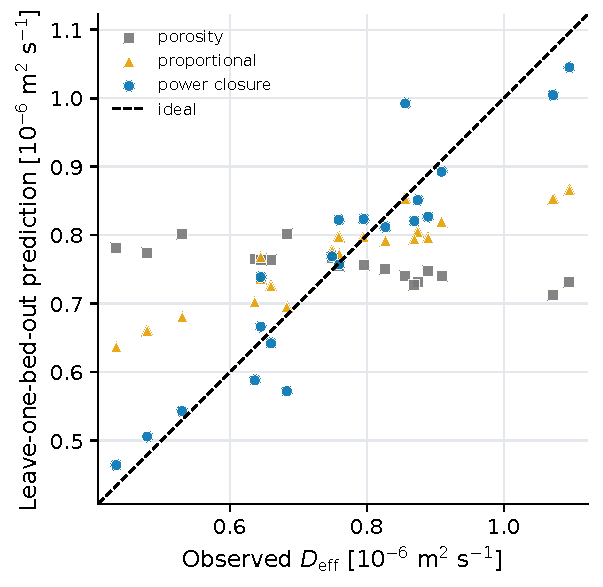
\includegraphics[width=\linewidth,height=0.69\textheight,keepaspectratio]{figures/fig_closure_held_out.pdf}
    \column{0.32\textwidth}
    \small
    \hi{Closures compared}
\[
\begin{aligned}
 D_{\rm eff}&=a_0+a_1\varepsilon_b,\\
 D_{\rm eff}&=\alpha D_{\rm access},\\
 \frac{D_{\rm eff}}{D_m}&=C\left(\frac{D_{\rm access}}{D_m}\right)^n.
\end{aligned}
\]
Fit on nineteen beds, then predict the remaining bed.
  \end{columns}
  \vspace{0.12cm}
  {\small\result{LOOCV $R^2$: power law $0.890$, proportional $0.555$, porosity $-0.234$.}}
  \note{We leave out one entire bed, fit each closure to the other nineteen, and predict the omitted diffusivity. Repeating this gives twenty held-out predictions. Blue circles show the power law, orange triangles show proportionality, and grey squares show porosity. Model form and diagnostic depth were compared within this ensemble, so these scores remain internal validation.}
\end{frame}

\begin{frame}{Accessibility remains correlated across diagnostic depths}
  \begin{columns}[c,onlytextwidth]
    \column{0.65\textwidth}
    \centering
    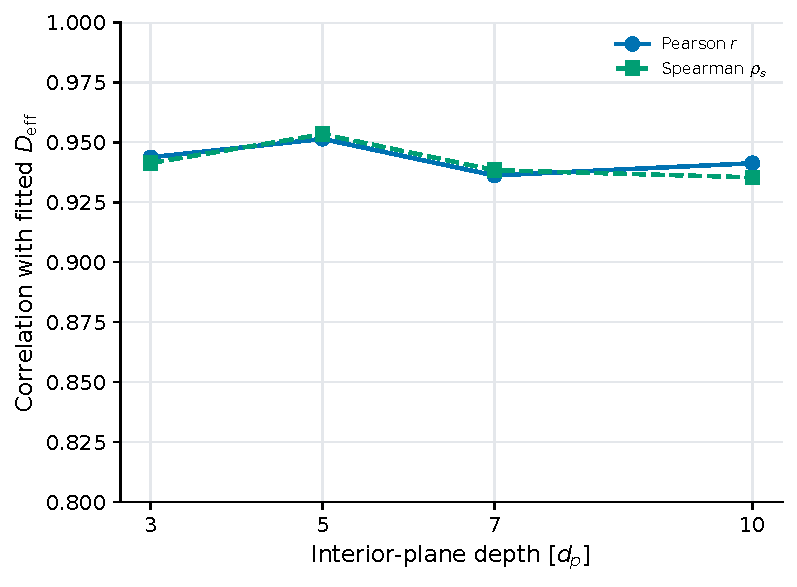
\includegraphics[width=\linewidth,height=0.69\textheight,keepaspectratio]{figures/fig_depth_correlations.pdf}
    \column{0.32\textwidth}
    \small
    \hi{Depth sensitivity}
\begin{itemize}
\item planes at $3$, $5$, $7$ and $10d_p$
\item Pearson: linear association
\item Spearman: rank association
\end{itemize}
\medskip
Depth is measured above each network's lowest pore.
  \end{columns}
  \vspace{0.12cm}
  {\small\result{Both correlations remain high across the tested depths.}}
  \note{The original descriptor places the diagnostic plane above the lowest pore in each network. We tested three, five, seven and ten particle diameters using that convention. Both linear and rank correlations remain high. These depths are not measured exactly from the physical bed bottom.}
\end{frame}

\begin{frame}{Predictive performance is stable across diagnostic depths}
  \begin{columns}[c,onlytextwidth]
    \column{0.65\textwidth}
    \centering
    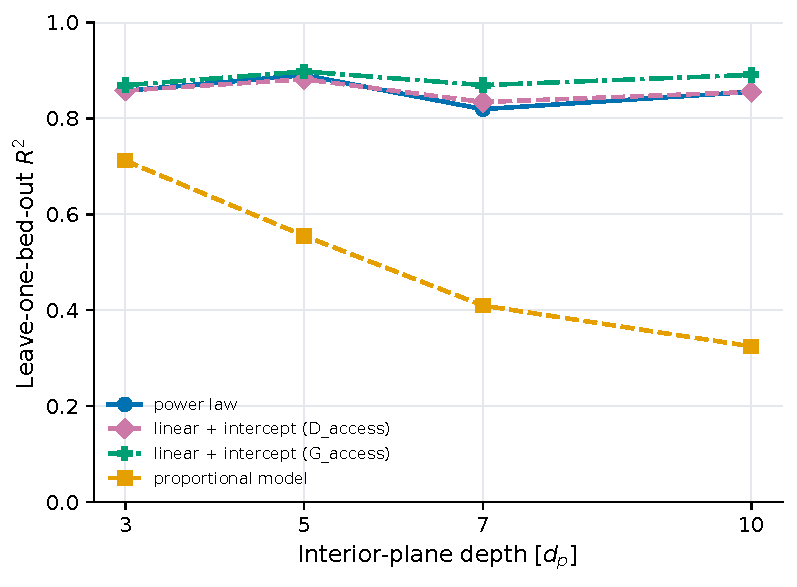
\includegraphics[width=\linewidth,height=0.69\textheight,keepaspectratio]{figures/fig_depth_prediction.pdf}
    \column{0.32\textwidth}
    \small
    \hi{Models in this comparison}
\begin{itemize}
\item linear model with intercept
\[D_{\rm eff}=aD_{\rm access}+b\]
\item proportional model
\[D_{\rm eff}=\alpha D_{\rm access}\]
\end{itemize}
\medskip
The $5d_p$ plane gives the highest linear-model score in this ensemble.
  \end{columns}
  \vspace{0.12cm}
  {\small\result{The linear model with intercept remains predictive from $3d_p$ to $10d_p$.}}
  \note{This plot compares affine and proportional closures at each depth. It does not plot the power-law score. Five particle diameters gives the best linear-model score among these tested depths. This sensitivity supports the association while independent beds are still needed to evaluate model and depth selection.}
\end{frame}

\section[Conclusions]{Conclusions and next steps}
\begin{frame}{}
\vfill
{\large\color{tumgray}Section 5 of 5}\par\vspace{0.4cm}
{\LARGE\color{tumblue}\textbf{Conclusions and next steps}}\par\vspace{0.5cm}
{\large What the evidence supports and what remains to validate}
\vfill
\note{What the evidence supports and what remains to validate.}
\end{frame}

\begin{frame}{What the present evidence establishes}
  \begin{FlexRow}{0.58\textheight}
    \Col{0.47}{
      \hi{Supported}
      \begin{itemize}
        \item porosity alone misses important packing variability
        \item inlet-connected topology controls transient utilization
        \item one $D_{\rm eff}$ reproduces each detailed curve accurately
        \item $D_{\rm access}$ provides an interpretable predictive closure
      \end{itemize}}
    \Col{0.47}{
      \hi{Not yet claimed}
      \begin{itemize}
        \item industrial breakthrough performance
        \item effects of flow, heat or water competition
        \item transfer to other bead sizes or $D_{\rm tube}/d_p$
        \item a universal power-law exponent
      \end{itemize}}
  \end{FlexRow}

  \vspace*{0.5cm}
  \result{The contribution is a structure-to-model closure for a controlled diffusion-driven adsorption problem.}
  \note{
    The present evidence supports four conclusions. Bulk porosity misses
    important differences among random packings. Inlet-connected topology
    explains a large part of the resulting variation. One optimized
    $D_{\rm eff}$ allows the 1D model to reproduce each detailed uptake curve
    accurately. Finally, $D_{\rm access}$ provides a cheap and interpretable
    input for predicting that coefficient.

    The scope must remain clear. We have not modelled an industrial
    breakthrough column with imposed flow. We have not included heat effects,
    water or competitive adsorption. We also have not demonstrated that the
    fitted power law transfers to other bead sizes or tube-to-particle ratios.
    The result is a validated structure-to-model closure for this controlled,
    diffusion-driven adsorption problem, rather than a universal adsorption
    correlation.
  }
\end{frame}

\begin{frame}{Pore accessibility retains what bulk porosity loses}
  \question{Equal void volume does not imply equal transport. How that void space connects to the inlet matters.}
  \vspace{0.55cm}
  \centering
  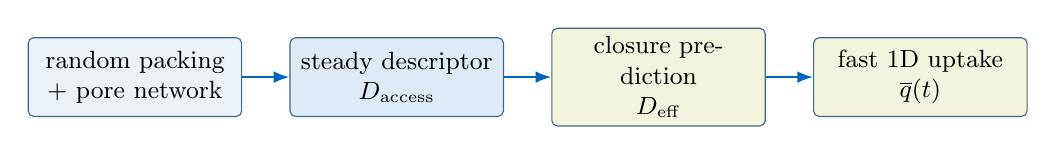
\begin{tikzpicture}[node distance=6mm,
    finalbox/.style={box,text width=2.5cm,minimum height=10mm}]
    \node[finalbox] (geom) {random packing\\+ pore network};
    \node[finalbox,right=of geom,fill=tumblue!13] (da) {steady descriptor\\$D_{\rm access}$};
    \node[finalbox,right=of da,fill=tumgreen!13] (de) {closure prediction\\$D_{\rm eff}$};
    \node[finalbox,right=of de,fill=tumgreen!13] (q) {fast 1D uptake\\$\overline q(t)$};
    \draw[arr] (geom)--(da);\draw[arr] (da)--(de);\draw[arr] (de)--(q);
  \end{tikzpicture}
  \vspace{0.65cm}
  \begin{columns}[T,onlytextwidth]
    \column{0.31\textwidth}\centering\hi{20 beds}\\controlled ensemble
    \column{0.31\textwidth}\centering\hi{1.58\%}\\mean reduction error
    \column{0.31\textwidth}\centering\hi{$R^2=0.890$}\\withheld-bed closure
  \end{columns}
  \note{
    The main message is that equal void volume does not imply equal transport.
    How the void space connects to the inlet matters. Starting from a random
    packing, we extract the pore network and calculate the steady accessibility
    descriptor. The fitted closure converts this descriptor into
    $D_{\rm eff}$, and the conservative 1D model uses that coefficient to
    predict the transient uptake.

    Across twenty controlled beds, porosity varied by only 0.55 percent while
    uptake varied much more strongly. The optimized 1D model reproduced the
    pore-network curves with a mean NRMSE of 1.58 percent. The accessibility
    power law achieved a leave-one-bed-out $R^2$ of 0.890. The practical outcome
    is therefore a fast transient model that retains a clear and measurable
    link to the underlying packing structure.
  }
\end{frame}
\end{document}
